\chapter{Quantum Computing}
\label{sec:quantum_computing}

This chapter gives an introduction to the field of \textit{Quantum Computation}. It covers the basics of qubits, quantum gates and circuits, and gives an overview of quantum complexity classes. The chapter is based on \cite{nielsen2002quantum}, which offers a profound introduction into the field.

\section{Qubits}

While classical computers harness classical physical phenomena like electrical current to perform calculations, quantum computers harness 
\textit{quantum mechanical} effects. The simplest quantum mechanical system is a quantum bit, or
\textit{qubit} for short. It is the fundamental building block of a quantum computer.

Mathematically, a qubit is a two-dimensional complex-valued unit vector,
also called the \textit{state vector} or \textit{wave function}:

\begin{equation}
  \label{eq:qubit1}
  \Ket{\psi} = \begin{pmatrix} \alpha \\ \beta \end{pmatrix}
\end{equation}

with \textit{amplitudes} $\alpha, \beta \in \mathbb{C}$ and $|\alpha|^2 + |\beta| ^2 = 1$ . 
Rewriting $\Ket{\psi}$ as

\begin{equation}
  \Ket{\psi} = e^{i \gamma} \left( \cos{\frac{\theta}{2}} \Ket{0} + e^{i \rho} \sin{\frac{\theta}{2}} \Ket{1} \right)
\end{equation}

with $\theta, \rho, \gamma \in \mathbb{R}$
allows an intuitive interpretation of a qubit as a point on the surface of the three-dimensional unit sphere.
This sphere is also called the \textit{Bloch Sphere} and is visualized in figure~\ref{fig:blochsphere}. The factor $e^{i \gamma}$ in front is called a
\textit{global phase} and can be ignored:

\begin{equation}
  \Ket{\psi} = \cos{\frac{\theta}{2}} \Ket{0} + e^{i \rho} \sin{\frac{\theta}{2}} \Ket{1}.
\end{equation}

\begin{figure}[H]
  \centering
  \begin{tikzpicture}

    % Define radius
    \def\r{3}

    % Bloch vector
    \draw (0,0) node[circle,fill,inner sep=1] (orig) {} -- (\r/3,0.7*\r) node[circle,fill,inner sep=0.7,label=right:$\Ket{\psi}$] (a) {};
    \draw[dashed] (orig) -- (\r/3,-\r/5) node (phi) {} -- (a);

    % Sphere
    \draw[line width=0.5mm] (orig) circle (\r);
    \draw[dashed, line width=0.5mm] (orig) ellipse (\r{} and \r/5);

    % Axes
    \draw[->] (orig) -- ++(-\r/2,-\r/3) node[below] (x) {$x$};
    \draw[->] (orig) -- ++(\r+0.5,0) node[right] (y) {$y$};
    \draw[->] (orig) -- ++(0,\r+0.5) node[above] (z) {$z$};

    % Basis States
    \filldraw[fill=white, line width=0.3mm] (0,\r) circle (0.15) node[label={[label distance=0.01mm]50:$\Ket{0}$}] (0) {};
    \filldraw[fill=white, line width=0.3mm] (0,-\r) circle (0.15) node[label={[label distance=0.01mm]325:$\Ket{1}$}] (1) {};

    % Angles
    \pic [draw=gray,text=gray,-,"$\phi$", angle radius=0.5cm] {angle = x--orig--phi};
    \pic [draw=gray,text=gray,-,"$\theta$", angle radius=1cm] {angle = a--orig--z};

  \end{tikzpicture}
  \caption[The Bloch Sphere]{Bloch Sphere representation of a qubit state $\Ket{\psi}$. $\Ket{\psi}$ points to an arbitrary direction on the three dimensional unit sphere.}
  \label{fig:blochsphere}
\end{figure}

The states on the north and south pole of the Bloch Sphere are called the
\textit{computational basis states}, defined as:

\begin{equation}
  \Ket{0} = \begin{pmatrix} 1 \\ 0 \end{pmatrix} \phantom{.}
\end{equation}

and

\begin{equation}
  \Ket{1} = \begin{pmatrix} 0 \\ 1 \end{pmatrix}.
\end{equation}

These states correspond to the classical states $0$ and $1$ of a classical bit. Thus, another way of writing the wave
function of a qubit, which is also the most practical one for quantum computation, is a linear combination of the
two computational basis states:

\begin{equation}
  \Ket{\psi} = \alpha \cdot \Ket{0} + \beta \cdot \Ket{1}.
\end{equation}

A qubit whose amplitudes $\alpha$ and $\beta$ are both non-zero is in a so-called \textit{superposition} of the two
computational basis states. A qubit in a superposition can be interpreted as being in both states $\Ket{0}$ and $\Ket{1}$ at the same time.
This property is one of the underlying reasons why the classical simulation of
quantum systems is computationally so hard, and it is one of the sources of the potential computational power of quantum computers.
Nevertheless, it is not possible to read the values of the amplitudes $\alpha$ and $\beta$
directly.

The qubit can only be in a superposition as long as it is completely isolated
from its environment. Such a state is called a \textit{coherent} state. As
soon as the qubit interacts with its environment, as it is necessary to read
its value, it collapses randomly into one of the two computational basis
states. All the information that was stored in the amplitudes gets lost in this process.

In a quantum computer, the qubits are in a coherent state, and potentially in a superposition, during the computation. At the end of the computation, a so-called
\textit{projective measurement} is performed to read the states of the individual qubits. A projective measurement is given
by \textit{operators} $\textbf{M} = \{M_i\}$, in this case $M_0 = \Ket{0}\Bra{0}$ and $M_1 = \Ket{1}\Bra{1}$. The probabilities $p(0)$ and $p(1)$ of observing a qubit in the $\Ket{0}$ or
$\Ket{1}$ state are then defined by the amplitudes:

\begin{align}
  p(0) &= \Bra{\psi} M_0^{\dagger}M_0 \Ket{\psi} \\
       &=  \Bra{\psi} M_0 \Ket{\psi} \\
       &= \alpha \Braket{0|0} \Bra{0} \alpha \Ket{0} + \beta \Braket{1|0} \Bra{0} \beta \Ket{1} \\
       &= \alpha^2 \Braket{0|0} \Braket{0|0} + \beta^2 \Braket{1|0} \Braket{0|1} \\
       &= \alpha^2
\end{align}

and

\begin{align}
  p(1) &= \Bra{\psi} M_1^{\dagger} M_1 \Ket{\psi} \\
       &= \Bra{\psi} M_1 \Ket{\psi} \\
       &= \alpha \Braket{0|1} \Bra{1} \alpha \Ket{0} + \beta \Braket{1|1} \Bra{1} \beta \Ket{1} \\
       &= \alpha^2 \Braket{0|1} \Braket{1|0} + \beta^2 \Braket{1|1} \Braket{1|1} \\
       &= \beta^2
\end{align}

as $M_i^{\dagger}M_i = M_i$ and $\Braket{i|j} = \delta_{ij}$.

After the measurement, the state of the qubit will be either

\begin{align}
  \Ket{\psi^{\dagger}} &= \frac{M_0 \Ket{\psi}}{\sqrt{p(0)}} \\
                       &= \frac{\Ket{0}\Bra{0}\left(\alpha \Ket{0} + \beta \Ket{1}\right)}{\sqrt{\alpha^2}} \\
                       &= \frac{\alpha \Ket{0}\Braket{0 | 0} + \beta \Ket{0} \Braket{ 0 | 1} }{\alpha} \\
                       &= \frac{\alpha \Ket{0}}{\alpha} \\
                       &= \Ket{0}
\end{align}

or

\begin{align}
  \Ket{\psi^{\dagger}} &= \frac{M_1 \Ket{\psi}}{\sqrt{p(1)}} \\
                       &= \frac{\Ket{1}\Bra{1}\left(\alpha \Ket{0} + \beta \Ket{1}\right)}{\sqrt{\beta^2}} \\
                       &= \frac{\alpha \Ket{1}\Braket{1 | 0} + \beta \Ket{1} \Braket{ 1 | 1} }{\beta} \\
                       &= \frac{\beta \Ket{1}}{\beta} \\
                       &= \Ket{1}
\end{align}

respectively, implying that the state of the qubit collapsed into one of the two computational
basis states. Thus, any successive measurement will result in the same outcome.
In order to perform multiple measurements on the same state, it has to be prepared multiple times.

Two special qubit states, which often occur in the domain of quantum computation, are the $\Ket{-}$ and $\Ket{+}$ state defined as:

\begin{equation}
  \Ket{-} = \frac{1}{\sqrt{2}} \cdot \Ket{0} - \frac{1}{\sqrt{2}} \cdot \Ket{1} \phantom{.}
\end{equation}

and

\begin{equation}
  \Ket{+} = \frac{1}{\sqrt{2}} \cdot \Ket{0} + \frac{1}{\sqrt{2}} \cdot \Ket{1}.
\end{equation}

Those states differ in a \textit{relative phase}. Both have the same measurement statistics, lying between the states $\Ket{0}$ and
$\Ket{1}$ on the Bloch Sphere:

\begin{align}
  p(0) &= \Bra{+} M_0 \Ket{+} \\
       &= \frac{1}{\sqrt{2}} \Braket{0|0} \Bra{0} \frac{1}{\sqrt{2}} \Ket{0} + \frac{1}{\sqrt{2}} \Braket{1|0} \Bra{0} \frac{1}{\sqrt{2}} \Ket{1} \\
       &= \frac{1}{2} \Braket{0|0} \Braket{0|0} + \frac{1}{2} \Braket{1|0} \Braket{0|1} \\
       &= \frac{1}{2}
\end{align}


and

\begin{align}
  p(1) &= \Bra{+} M_1 \Ket{+} \\
       &= \frac{1}{\sqrt{2}} \Braket{0|1} \Bra{1} \frac{1}{\sqrt{2}} \Ket{0} + \frac{1}{\sqrt{2}} \Braket{1|1} \Bra{1} \frac{1}{\sqrt{2}} \Ket{1} \\
       &= \frac{1}{2} \Braket{0|1} \Braket{1|0} + \frac{1}{2} \Braket{1|1} \Braket{1|1} \\
       &= \frac{1}{2}
\end{align}



for the $\Ket{+}$ state. The same probabilities hold for the
$\Ket{-}$ state.
Again, the state will be destroyed on measurement and be either $\Ket{0}$ or $\Ket{1}$ afterward, depending on the measurement outcome.

\section{Multiple Qubits and Entanglement}
\label{sec:multiplequbitsandentanglement}

The state vector of a single qubit lies in a two-dimensional 
space, assigning a complex-valued amplitude to each of the both possible measurement outcomes
$\Ket{0}$ and $\Ket{1}$. The state vector of a multi-qubit system is defined by
the \textit{tensor product} of the state vectors of the individual subsystems.
For a two-qubit system consisting of $\Ket{\psi_1} = \alpha_1 \Ket{0} + \beta_1
\Ket{1}$ and $\Ket{\psi_2} = \alpha_2 \Ket{0} + \beta_2 \Ket{1}$, the state vector
is given by:

\begin{align}
  \Ket{\psi_{1,2}} &= \Ket{\psi_1} \otimes \Ket{\psi_2} \\
                   &= (\alpha_1 \Ket{0} + \beta_1 \Ket{1}) \otimes (\alpha_2 \Ket{0} + \beta_2 \Ket{1}) \\
                   &= \alpha_1 \alpha_2 \Ket{0}\Ket{0} + \alpha_1 \beta_2 \Ket{0} \Ket{1} + \beta_1 \alpha_2 \Ket{1} \Ket{1} + \beta_1 \beta_2 \Ket{1} \Ket{1} \\
                   &= \alpha_1 \alpha_2 \Ket{00} + \alpha_1 \beta_2 \Ket{01} + \beta_1 \alpha_2 \Ket{10} + \beta_1 \beta_2 \Ket{11} \\
                   &= \alpha_1 \alpha_2 \Ket{0} + \alpha_1 \beta_2 \Ket{1} + \beta_1 \alpha_2 \Ket{2} + \beta_1 \beta_2 \Ket{3},
\end{align}

where $\Ket{0} = \Ket{00}$, $\Ket{1} = \Ket{01}$, $\Ket{2} = \Ket{10}$
and $\Ket{3} = \Ket{11}$. In general, the wave function of a
n-qubit system is given by a $2^n$ dimensional vector:

\begin{equation}
  \Ket{\psi} = \sum_{i=0}^{2^n}a_i \Ket{i}.
\end{equation}

Therefore, a classical simulation of a n-dimensional qubit system has to keep
track of $2^n$ complex amplitudes. This makes it impossible to simulate quantum
systems above a certain size. For the classical simulation of a system
consisting of 500 qubits, the state vector's dimension is already larger
than the number of atoms in the universe.  

As in the single-qubit case, the probability to observe state $\Ket{n}$ is
given by $a_n^2$. It is also possible to only measure a subset of the qubits,
leaving the other qubits in the normalized state:

\begin{equation}
  \Ket{\psi\prime} = \frac{(M_m \otimes I) \Ket{\psi}}{\sqrt{p(m)}}.
\end{equation}

A phenomenon that can appear in multi-qubit systems is
\textit{entanglement}. Consider for instance the two-qubit state

\begin{equation}
  \Ket{\psi} = \frac{\Ket{00} + \Ket{11}}{\sqrt{2}}.
\end{equation}

This state can be created with a very simplistic quantum program as shown later in
section~\ref{sec:quantum_circuits}.
Note that this state is a proper two-qubit state as it fulfills the
normalization property
$a_{00}^2 + a_{11}^2 = \frac{1}{\sqrt{2}}^2 + \frac{1}{\sqrt{2}}^2 = \frac{1}{2}
+ \frac{1}{2} = 1$.

Nevertheless, there are no two single-qubit states $\Ket{a}$
and $\Ket{b}$ such that $\Ket{\psi} = \Ket{a} \Ket{b}$. The two qubits of
$\Ket{\psi}$ are \textit{entangled} with each other. Measuring one of the qubits
immediately determines the state of the other qubit, i.e. measuring the first
qubit as $\Ket{0}$ happens with probability:

\begin{align}
  p_1(0) &= \Bra{\psi} (M_0 \otimes I)^{\dagger} (M_o \otimes I) \Ket{\psi} \\
         &= \frac{1}{\sqrt{2}} \Bra{00} \frac{1}{\sqrt{2}} \Ket{00} \\
         &= \frac{1}{2},
\end{align}

leaving the system in the post-measurement state:

\begin{align}
  \Ket{\psi\prime} &= \frac{(M_0 \otimes I) \psi}{\sqrt{p_1(0)}} \\
                   &= \frac{\frac{1}{\sqrt{2}} \Ket{00}}{\frac{1}{\sqrt{2}}} \\
                   &= \Ket{00}.
\end{align}

The same maths apply for the case of measuring the first qubit as $\Ket{1}$.

Even if the state of the second qubit is not determined before, it will be
either $\Ket{0}$ or $\Ket{1}$ from the moment on the \textit{other} qubit has been measured.

The exponential growth of the state space dimension and entanglement are two 
properties of quantum systems which make them hard to simulate
classically.
Known quantum algorithms with quantum speedups like Shor's algorithm
create entanglement in smart ways to perform calculations which seem
to be impossible for classical computers.

\section{Quantum Gates}

It is physically possible to modify the state vector of a quantum system, even
when it is in a coherent state. This opens the theoretical possibility to perform
calculations based on the laws of quantum physics and build quantum computers.

The quantum state can be modified through \textit{quantum gates}. 
Quantum physics allows the gates only to be linear and reversible. Thus,
quantum gates can be mathematically described as unitary matrices. Gates vary in the number of
qubits on which they act and the effects they have on the qubits' state.

\subsection{Single-Qubit Gates}

Single-qubit gates are linear mappings that can be applied to the state vector
of a single qubit. Mathematically, single-qubit gates can be described by $2
\times 2$ unitary matrices. The fact that these matrices are unitary guarantees that
the state $\Ket{\phi} = G \Ket{\psi}$ after gate $G$ has been applied to state $\Ket{\psi}$ is a
proper quantum state which preserves the normalization constraint
$\alpha_{\Ket{\phi}}^2 + \beta_{\Ket{\phi}}^2 = 1$.

An example of a single-qubit gate is the NOT or $X$ gate, also denoted as:

\begin{figure}[h]
  \centering
  \mbox{
    \Qcircuit @C=1em @R=1em {
      & \gate{X} & \qw
    }
  }
\end{figure}

or

\begin{figure}[h]
  \centering
  \mbox{
    \Qcircuit @C=1em @R=1em {
      & \targ & \qw
    }
  }.
\end{figure}

The $X$ gate is the quantum analog of
the classical NOT gate. Like the classical version, the $ X $ gate swaps the
states $\Ket{0}$ and $\Ket{1}$ when applied to them. It is even more general, as it maps a
single-qubit state of the form

\begin{equation}
    \Ket{\psi} = \alpha \Ket{0} + \beta \Ket{1}
\end{equation}

to the state 

\begin{equation}
  \Ket{\phi} = \beta \Ket{0} + \alpha \Ket{1}
\end{equation}

by swapping the amplitudes for $\Ket{0}$ and $\Ket{1}$. The $X$ gate has the
following matrix representation:

\begin{equation}
  X =
  \begin{pmatrix}
    0 & 1 \\
    1 & 0
    \end{pmatrix}.
\end{equation}

A single-qubit gate is applied to a quantum state by matrix multiplication:

\begin{align}
  \Ket{\phi} &= X \Ket{\psi} \\
             &=
               \begin{pmatrix}
                 0 & 1 \\
                 1 & 0
               \end{pmatrix}
                \Ket{\psi} \\
             &= \begin{pmatrix}
                 0 & 1 \\
                 1 & 0
               \end{pmatrix}
                \begin{pmatrix}
                  \alpha \\
                  \beta
                \end{pmatrix} \\
             &= \begin{pmatrix}
                 \beta \\
                 \alpha
               \end{pmatrix}
\end{align}

Another example of a single-qubit gate without any classical analog is the
\textit{Hadamard gate} or $H$ gate, described by the unitary:

\begin{equation}
  H = \frac{1}{\sqrt{2}}
  \begin{pmatrix}
    1 & 1 \\
    1 & -1
  \end{pmatrix}.
\end{equation}

Notice that the H gate is a unitary as it is reversible:

\begin{equation}
   H^{\dagger} H = I.
\end{equation}

The Hadamard gate maps between the so-called $Z$ and $X$ bases, mapping the
states:

\begin{align}
  H \Ket{0} &= \Ket{+} \\
  H \Ket{1} &= \Ket{-} \phantom{.}
\end{align}

and back

\begin{align}
  H \Ket{+} &= \Ket{0} \\
  H \Ket{-} &= \Ket{1}.
\end{align}

The Hadamard gate is a good example of how the Bloch Sphere visualization can help to understand a qubit state's transformation. The application of the Hadamard gate to the $\Ket{+}$ is shown in figure~\ref{fig:blochH}.

\begin{figure}[H]
  \centering
  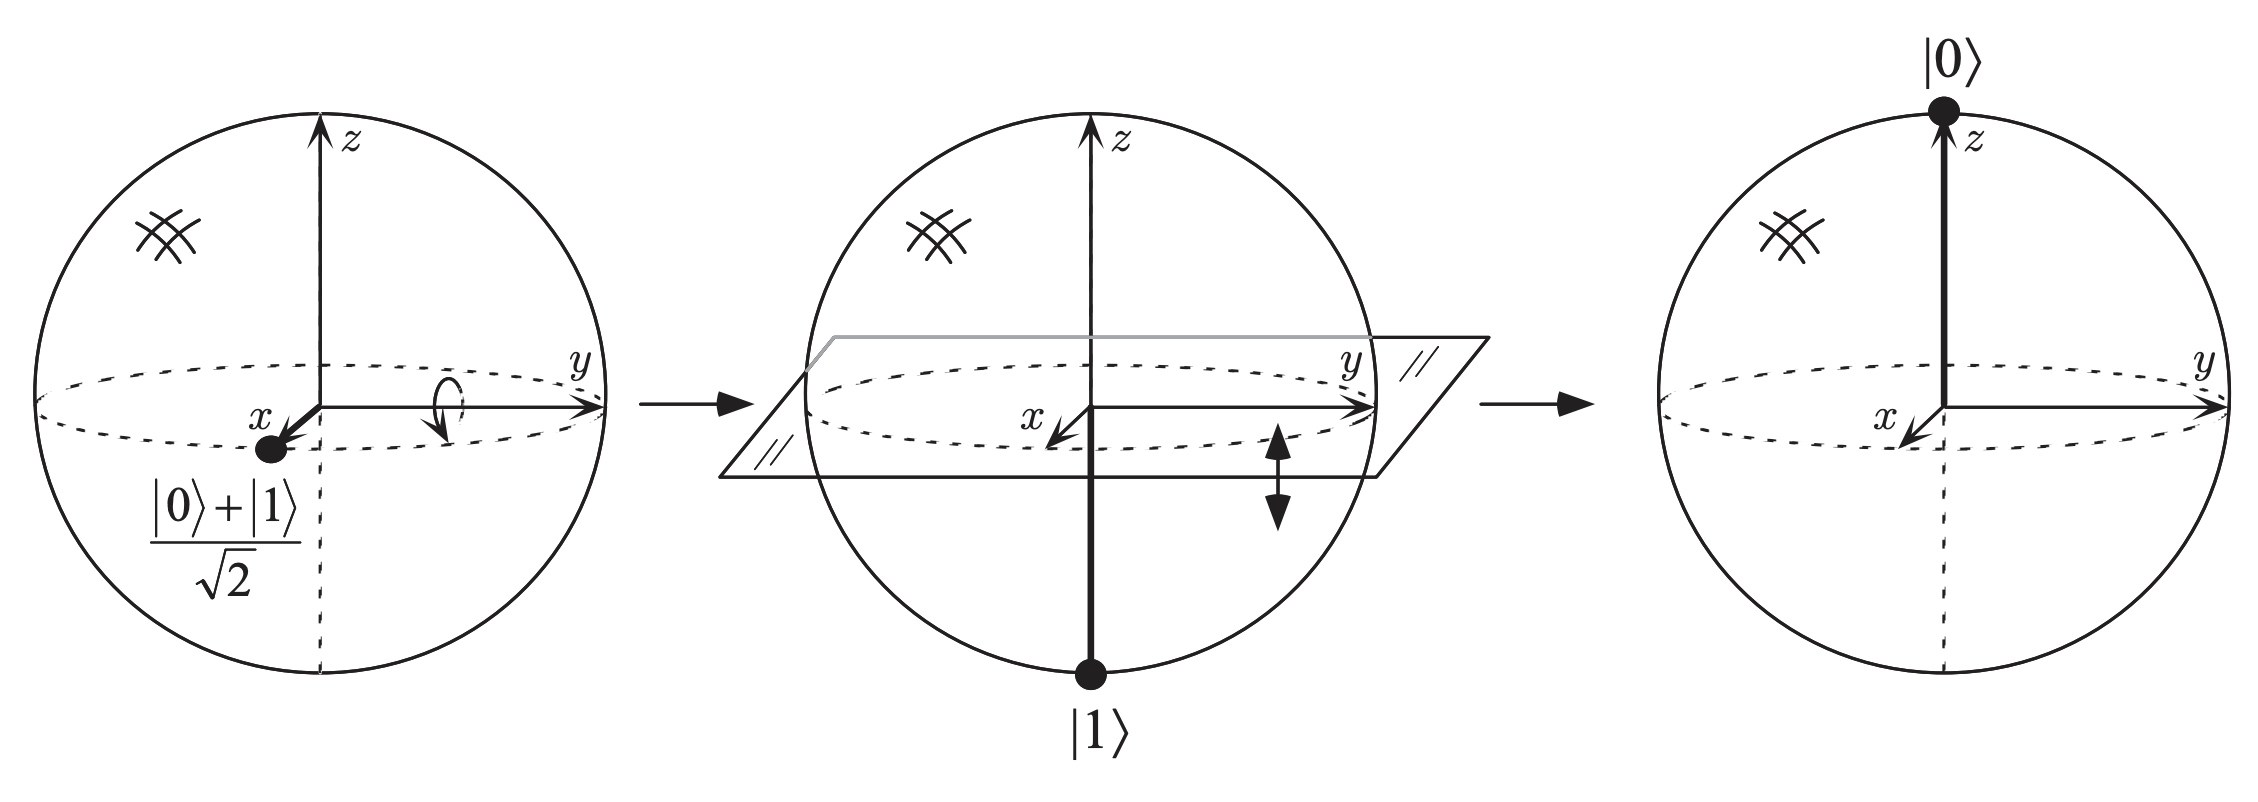
\includegraphics[width=\textwidth]{figures/hadamard}
  \caption[Hadamard Visualization]{Visualization of the Hadamard gate on the Bloch sphere, acting on the $\Ket{+}$ state. Graphic taken from \cite{nielsen2002quantum}.}
  \label{fig:blochH}
\end{figure}

An overview of some common single-qubit gates is given in figure \ref{fig:singlegates}.

\begin{table}[H]
  \centering
  \begin{tabular}{c c c}
    Operator & Gate & Matrix \\[20pt]
    $X$ &  \Qcircuit @C=1em @R=.7em { & \gate{X} & \qw } & $\begin{pmatrix} 0 & 1 \\ 1 & 0\end{pmatrix}$ \\[20pt]
    $Y$ &  \Qcircuit @C=1em @R=.7em { & \gate{Y} & \qw } & $\begin{pmatrix} 0 & -i \\ i & 0\end{pmatrix}$ \\[20pt]
    $Z$ &  \Qcircuit @C=1em @R=.7em { & \gate{Z} & \qw } & $\begin{pmatrix} 1 & 0 \\ 0 & -1\end{pmatrix}$ \\[20pt]
    $H$ &  \Qcircuit @C=1em @R=.7em { & \gate{H} & \qw } & $\frac{1}{\sqrt{2}} \begin{pmatrix} 1 & 1 \\ 1 & -1\end{pmatrix}$ \\[20pt]
    $S$ &  \Qcircuit @C=1em @R=.7em { & \gate{S} & \qw } & $\begin{pmatrix} 1 & 0 \\ 0 & i\end{pmatrix}$ \\[20pt]
    $T$ &  \Qcircuit @C=1em @R=.7em { & \gate{T} & \qw } & $\begin{pmatrix} 1 & 0 \\ 0 & e^{i\frac{\pi}{2}}\end{pmatrix}$ \\[20pt]
  \end{tabular}
  \caption[Overview of common single-qubit gates]{Overview of common single-qubit gates.}
  \label{fig:singlegates}
\end{table}

There are indefinitely many possible quantum gates in theory. Still, 
a universal finite gate set 
consisting of a few gates is sufficient to construct arbitrary unitary
transformations \cite{kitaev2002classical}. This is the same as in the classical case where NAND gates
suffice to build up arbitrary classical computation circuits \cite{sheffer13transactions} and 
 good news for the fabrication of quantum computers with reusable components.

Nevertheless, single-qubit gates are not sufficient to build all possible unitary transformations on multi-qubit systems. 
For this purpose, multi-qubit gates are a necessity.

\subsection{Multi-Qubit Gates}

Single-qubit gates are not sufficient to create universal gate sets for quantum
computation. In order to run arbitrary quantum programs, multi-qubit gates such as
 \textit{controlled} gates are needed.
Controlled quantum gates are simple extensions of single-qubit gates. Every single-qubit gate can be implemented as a controlled 
version of it with one \textit{control} and one \textit{target} qubit. Only if
the control qubit is in the $\Ket{1}$ state, the gate is applied to the target
qubit. As the control qubit can be in a superposition state, it is possible to apply and not apply the gate to the target qubit at the same time.

The prototypical two-qubit gate is the controlled NOT or CNOT gate. It is the controlled version of the 
$X$ gate described before. As the CNOT gate acts on a two-qubit state, it can be described by 
a $4 \times 4$ unitary matrix. Each column describes the mapping of one of the four base
state $\Ket{00}$, $\Ket{01}$, $\Ket{10}$ and $\Ket{11}$. 
The matrix representation of the CNOT gate is the following:

\begin{equation}
  CNOT = \begin{pmatrix}
    1 & 0 & 0 & 0 \\
    0 & 1 & 0 & 0 \\
    0 & 0 & 0 & 1 \\
    0 & 0 & 1 & 0
    \end{pmatrix}.
\end{equation}

The matrix can be read as follows: The first two columns describe that the vectors $\Ket{00}$ and $\Ket{01}$ will not change when the gate is applied to these states. Only when the first qubit is in the $\Ket{1}$ state, will the state of the second qubit be swapped. Thus $\Ket{10}$ will be mapped to $\Ket{11}$ and $\Ket{11}$ to $\Ket{10}$. 

This shows how the matrix representation of generalized two-qubit gates can be derived: As long as the control qubit is off, it does not affect the state. Thus, the controlled gate matrix is the same as the identity with 1s on the diagonal and 0s elsewhere in the upper left corner. Only when the first qubit is in the $\Ket{1}$ state, the matrix differs from the identity. For example, the 
controlled version of the $Z$ gate:

\begin{equation}
  Z = \begin{pmatrix}
    1 & 0 \\
    0 & -1
    \end{pmatrix}
\end{equation}

is given by:

\begin{equation}
    CZ = \begin{pmatrix}
      1 & 0 & 0 & 0 \\
      0 & 1 & 0 & 0 \\
      0 & 0 & 1 & 0 \\
      0 & 0 & 0 & -1
      \end{pmatrix}.
\end{equation}

A controlled gate $G$ is represented by a vertical line ending in a black dot
indicating the control qubit:

\begin{figure}[h]
  \centering
  \mbox{
    \Qcircuit @C=1em @R=1em {
      &  \ctrl{1} & \qw \\
      &  \gate{G} & \qw
    }
  }
\end{figure}

With two-qubit operations at hand, it is possible to build a universal gate set. A commonly used gate set 
is the so-called \textit{Clifford + T} set, consisting of the gates $CNOT$, $H$, $S$ and
$T$ \cite{gottesman1998heisenberg}. The Solovay-Kitaev theorem \cite{kitaev2002classical} guarantees that this set can efficiently
approximate any unitary operation. In this study, another universal gate set will be used, 
composed of the $CZ$, $\sqrt{X}$, $\sqrt{Y}$ and $T$ gates \cite{martines2019supremacy}.

\section{Quantum Circuits}
\label{sec:quantum_circuits}

The standard model for computation in theoretical computer science is the Turing Machine \cite{10.1112/plms/s2-42.1.230}. Invented by 
Alan Turing in 1936, it is a powerful tool to understand the limits of (classical) 
computation. The
theoretical nature of the Turing machine gives it unlimited computational
resources, such as infinite memory, which do not reflect the properties of realizable
computer architectures.

Another computation model that does not suffer from the gap between theory
and practice is the \textit{circuit model} \cite{10.5555/522806}. In the classical circuit model, each bit is represented by a wire, and operations (or gates) are represented by different shapes acting on those wires. The circuit model is as powerful as a Turing Machine. It is the model of choice in quantum computing.

Quantum programs are described by quantum circuits. Each qubit is represented 
by a wire and each gate by a rectangular on those wires. Figure~\ref{fig:circuit0} describes a very simple quantum circuit which flips a single
qubit initialized in the $\Ket{0}$ state by applying a $X$ gate before
measuring it.

\begin{figure}[h]
  \centering
  \mbox{
    \Qcircuit @C=1em @R=1em {
      &  \lstick{\Ket{0}} & \qw & \gate{X} & \qw & \meter{0/1} 
    }
  }
  \caption[A Simple Quantum Circuit]{A simple quantum circuit applying an $X$ gate to a qubit initialized in the $\Ket{0}$ state before measuring it.}
  \label{fig:circuit0}
\end{figure}

The circuit is being read from left to right. Important to note is that
for calculating the resulting state, the matrix representation of the
gates are multiplied from the left side to the current state $\Ket{\psi}$.
In the example above the final state of the program represented at the end of the circuit is:

\begin{align}
  \Ket{\phi} &= X \Ket{\psi} \\
             &=
               \begin{pmatrix}
                 0 & 1 \\
                 1 & 0
               \end{pmatrix}
                     \Ket{\psi} \\
             &= \begin{pmatrix}
               0 & 1 \\
               1 & 0
             \end{pmatrix}
                   \begin{pmatrix}
                     \alpha \\
                     \beta
                   \end{pmatrix} \\
             &= \begin{pmatrix}
               \beta \\
               \alpha
             \end{pmatrix}.
\end{align}

In practice, circuits consist of several qubits with multiple gates applied
to them. It is possible to apply gates to different qubits sequentially as well
as in parallel, as demonstrated in figure~\ref{fig:circuit1}:

\begin{figure}[H]
  \centering
  \mbox{
    \Qcircuit @C=1em @R=1em {
      & \lstick{\Ket{0}} & \gate{H} & \gate{Z} & \qw & \gate{H} & \qw & \meter{0/1} \\
      & \lstick{\Ket{0}} & \qw & \gate{X} & \qw & \ctrl{-1} & \qw & \meter{0/1}
    }
  }
  \caption[A Quantum Circuit Acting on two Qubits]{A quantum circuit acting on two qubits. The effect of parallel applications of single-qubit gates is defined by the tensor product of the gates.}
  \label{fig:circuit1}
\end{figure}

Note that, when calculating the state of the quantum program above, the state of the system 
is given by the tensor product of the individual qubit states.
For the circuit from figure \ref{fig:circuit1}, the initial state $\Ket{\psi_{init}}$ before any gate has been applied 
is:

\begin{align}
    \Ket{\psi_{init}} &= \Ket{0} \otimes \Ket{0} \\
                      &= \begin{pmatrix} 1 \\ 0 \end{pmatrix} \otimes \begin{pmatrix} 1 \\ 0 \end{pmatrix} \\
                      &= \begin{pmatrix} 1 \\ 0 \\ 0 \\ 0 \end{pmatrix} \\
                      &= \Ket{00}. 
\end{align}

When a gate gets applied to only a subset of the qubits, as in the case of the
first $H$ gate in the circuit above, the unitary applied to the multi-qubit state is
implicitly the tensor product of the gate on that qubit and identity matrices on the
remaining qubits. For the given circuit, the state $\Ket{\psi_{H_1}}$ after the
first $H$ gate on the first qubit is calculated as: 

\begin{align}
  \Ket{\psi_{H_1}}  &= (H \otimes I) \Ket{00} \\
                   &= \left(\frac{1}{\sqrt{2}} \begin{pmatrix} 1 & 1 \\ 1 & -1 \end{pmatrix} \otimes \begin{pmatrix} 1 & 0 \\ 0 & 1 \end{pmatrix}\right) \Ket{00} \\
                    &= \frac{1}{\sqrt{2}} \begin{pmatrix} 1 & 0 & 1 & 0 \\ 0 & 1 & 0 & 1 \\ 1 & 0 & -1 & 0 \\ 0 & 1 & 0 & -1 \end{pmatrix} \Ket{00} \\
                    &= \frac{1}{\sqrt{2}} \begin{pmatrix} 1 & 0 & 1 & 0 \\ 0 & 1 & 0 & 1 \\ 1 & 0 & -1 & 0 \\ 0 & 1 & 0 & -1 \end{pmatrix} \begin{pmatrix} 1 \\ 0 \\ 0 \\ 0 \end{pmatrix} \\
                    &= \frac{1}{\sqrt{2}} \begin{pmatrix} 1 \\ 0 \\ 1 \\ 0 \end{pmatrix} \\
                    &= \Ket{+0}.
\end{align}

As expected, applying a $H$ gate to the first
qubit, it should be in the $\Ket{+}$ state while the second qubit remains in
the $\Ket{0}$ state.

Similar to the first gate, the unitary applied to the state, when multiple
gates are applied to different qubits at the same time, is constructed by the
tensor product of those gates. The resulting state $\Ket{\psi_{Z_1X_2}}$ after the $Z$
gate is applied to the first qubit, and the $X$ gate is applied to the second qubit, is
calculated as:

\begin{align}
  \Ket{\psi_{Z_1X_2}}  &= (Z \otimes X) \Ket{+0} \\
                    &= \left(\begin{pmatrix} 1 & 0 \\ 0 & -1 \end{pmatrix} \otimes \begin{pmatrix} 0 & 1 \\ 1 & 0 \end{pmatrix}\right) \Ket{+0} \\
                    &= \begin{pmatrix} 0 & 1 & 0 & 0 \\ 1 & 0 & 0 & 0 \\ 0 & 0 & 0 & -1 \\ 0 & 0 & -1 & 0 \end{pmatrix} \Ket{+0} \\
                    &= \begin{pmatrix} 0 & 1 & 0 & 0 \\ 1 & 0 & 0 & 0 \\ 0 & 0 & 0 & -1 \\ 0 & 0 & -1 & 0 \end{pmatrix} \begin{pmatrix} \frac{1}{\sqrt{2}} \\ 0 \\ \frac{1}{\sqrt{2}} \\ 0 \end{pmatrix} \\
                    &= \begin{pmatrix} 0 \\ \frac{1}{\sqrt{2}} \\ 0 \\ -\frac{1}{\sqrt{2}} \end{pmatrix} \\
                    &= \Ket{-1}.
\end{align}

Accordingly, applying a $Z$ gate to the $\Ket{+}$
state brings the first qubit to the $\Ket{-}$ state, while the $X$ gate on the second qubit moves the qubit state from the $\Ket{0}$ to the $\Ket{1}$ state.

The final state $\Ket{\psi_{final}}$ of the circuit is calculated by applying the $4 \times 4$ matrix
representation of the controlled $H$ gate to $\Ket{-1}$. In this case, the second
qubit is the controlled qubit:

\begin{align}
  \Ket{\psi_{final}}    &= CH \Ket{-1} \\
                        &= \begin{pmatrix} 1 & 0 & 0 & 0 \\ 0 & \frac{1}{\sqrt{2}} & 0 & \frac{1}{\sqrt{2}} \\ 0 & 0 & 1 & 0 \\ 0 & \frac{1}{\sqrt{2}} & 0 & -\frac{1}{\sqrt{2}} \end{pmatrix} \Ket{-1} \\
                       &= \begin{pmatrix} 1 & 0 & 0 & 0 \\ 0 & \frac{1}{\sqrt{2}} & 0 & \frac{1}{\sqrt{2}} \\ 0 & 0 & 1 & 0 \\ 0 & \frac{1}{\sqrt{2}} & 0 &  -\frac{1}{\sqrt{2}} \end{pmatrix} \begin{pmatrix} 0 \\ \frac{1}{\sqrt{2}} \\ 0 \\ -\frac{1}{\sqrt{2}} \end{pmatrix} \\
                       &= \begin{pmatrix} 0 \\ 0 \\ 0 \\ 1 \end{pmatrix} \\
                       &= \Ket{11}.
\end{align}

The first qubit has been swapped from the $\Ket{-}$ to the $\Ket{1}$ state as the
second qubit is in the $\Ket{1}$ state and the $H$ gate has been applied.
The circuit \ref{fig:circuit1} thus maps the initial state $\Ket{00}$ to $\Ket{11}$.

Another simple quantum circuit, which entangles two qubits with each other, is shown in figure \ref{fig:circuit2}.

\begin{figure}[H]
  \centering
  \mbox{
    \Qcircuit @C=1em @R=1em {
      & \lstick{\Ket{0}} & \gate{H} & \ctrl{1} & \qw & \meter{0/1} \\
      & \lstick{\Ket{0}} & \qw & \targ & \qw & \meter{0/1}
    }
  }
  \caption[Bell State Creation Circuit]{A quantum circuit to create maximally entangled 2-qubit states.}
  \label{fig:circuit2}
\end{figure}

The Hadamard gate on the first qubit maps the system from the initial $\Ket{00}$
into the $\Ket{+0}$ state. Afterward, the first qubit, which is currently
between the $\Ket{0}$ and $\Ket{1}$ state on the Bloch Sphere, is used as the
control qubit in the $CNOT$ gate. This has an interesting effect on the second qubit,
as the $X$ gate is applied and not applied at the same time, entangling
the two qubits with each other. The final state before measurement is
$\frac{\Ket{00} + \Ket{11}}{2}$, which has been discussed in section~\ref{sec:multiplequbitsandentanglement}.
This state is also known as one of the four \textit{Bell states}. They represent maximally
entangled two-qubit states. Moreover, they play an important role in the analysis of
\textit{quantum communication}.

The quantum circuit demonstrates how entanglement can be created by applying controlled gates with qubits in superposition states.
Entanglement plays an essential role in the construction of so-called \textit{random
quantum circuits} in recent quantum supremacy experiments.


\section{Quantum Computational Complexity}
\label{sec:quantum_computational_complexity}

It is essential to understand the theoretical capabilities and limitations of quantum computers to discover for which kind of problems
they provide advantages over classical computers. 

For many years, it has been assumed that the extended Church Turing thesis holds true. It states that a probabilistic
Turing machine can efficiently simulate any realistic model of computation. The thesis is challenged by quantum computers, because they can potentially solve specific problems exponentially faster than classical computers \cite{feynman1982simulating}.

The class of problems which can be solved efficiently by a quantum
computer is called \textbf{BQP}, shorthand for \textit{bounded-error quantum
  polynomial time} \cite{Bernstein93quantumcomplexity}. A decision problem is in \textbf{BQP} if there exists a quantum
program that solves the decision problem in 2/3 of the cases and runs in
polynomial time. This is the quantum analog of the \textit{bounded-error
  probabilistic polynomial time} or \textbf{BPP} \cite{gill1977computational}, which is decidable by a
probabilistic Turing machine in polynomial time and widely believed to be the same as
\textbf{P}.

Currently, there are a few problems known to be in \textbf{BQP}, which are suspected not to be in \textbf{P}, providing evidence for the superiority of quantum computers. One
of these problems is \textit{factorization}, the problem of decomposing a
composite integer into its prime factors. This problem has been known to be in
\textbf{NP} before. Though, it is also known that factorization is not an \textbf{NP}-hard problem, indicating that quantum computers are not able to provide
an exponential speedup for every problem that is not efficiently solvable on a
classical computer. Indeed, classical algorithms might even exist, which can
solve factorization on a classical computer efficiently, which have not been
discovered yet.

While \textbf{BQP} includes \textbf{P} and intersects with \textbf{NP}, it can be shown that it is strictly
included in \textbf{PSPACE} \cite{Bernstein93quantumcomplexity}. The relationship of these complexity classes is visualized
in figure \ref{fig:complexityclasses}.

\begin{figure}[H]
  \centering
  \begin{tikzpicture}

    \draw[line width=0.5mm] (orig) circle (1.25);
    \draw[dashed, line width=0.5mm] (orig) ellipse (2.05 and 1.35);
    \draw[line width=0.5mm] (0,0.5) circle (2);
    \draw[line width=0.5mm] (0,1) circle (2.5);

    \draw (0,0) node {\large \textbf{P}};
    \draw (0,2) node {\large \textbf{NP}};
    \draw (0,2.9) node {\large \textbf{PSPACE}};
    \draw (2.5,-1) node {\large \textbf{BQP?}};

  \end{tikzpicture}
  \caption[Relation of Complexity Classes to each other]{Relation of Complexity Classes to each other.}
  \label{fig:complexityclasses}
\end{figure}

While it is hard to prove some fundamental relationships between complexity
classes like the famous $\mathbf{P} \stackrel{?}{=} \mathbf{NP}$ problem, it is believed that quantum computers
can solve specific problems with practical applications like integer factorization \cite{shor1997factorisation} or the simulation of
quantum systems \cite{feynman1982simulating} exponentially faster than classical computers.

The moment
in time a physical quantum computer can outperform a classical computer
on a specific problem for the first time has been coined by John Preskill in
2012 as \textit{quantum supremacy} \cite{preskill2012quantum}. Recently, Google announced their quantum
supremacy results with a 54 qubit quantum computer, providing the first physical evidence that it
might be possible to build quantum computers with advantages over classical
computers \cite{martines2019supremacy}.